%%%%%%%%%%%%%%%%%%%%%%%%%%%%%%%%%%%%%%%%%
% Jacobs Landscape Poster
% LaTeX Template
% Version 1.0 (29/03/13)
%
% Created by:
% Computational Physics and Biophysics Group, Jacobs University
% https://teamwork.jacobs-university.de:8443/confluence/display/CoPandBiG/LaTeX+Poster
% 
% Further modified by:
% Nathaniel Johnston (nathaniel@njohnston.ca)
%
% This template has been downloaded from:
% http://www.LaTeXTemplates.com
%
% License:
% CC BY-NC-SA 3.0 (http://creativecommons.org/licenses/by-nc-sa/3.0/)
%
%%%%%%%%%%%%%%%%%%%%%%%%%%%%%%%%%%%%%%%%%

%----------------------------------------------------------------------------------------
%	PACKAGES AND OTHER DOCUMENT CONFIGURATIONS
%----------------------------------------------------------------------------------------

\documentclass[final,8pt]{beamer} % Font size here!!

\usepackage[scale=1]{beamerposter} % Use the beamerposter package for laying out the poster

\usetheme{confposter} % Use the confposter theme supplied with this template

\setbeamercolor{block title}{fg=ngreen,bg=white} % Colors of the block titles
\setbeamercolor{block body}{fg=black,bg=white} % Colors of the body of blocks
\setbeamercolor{block alerted title}{fg=white,bg=dblue!50} % Colors of the highlighted block titles
\setbeamercolor{block alerted body}{fg=black,bg=dblue!10} % Colors of the body of highlighted blocks
% Many more colors are available for use in beamerthemeconfposter.sty

%-----------------------------------------------------------x   
% Define the column widths and overall poster size
% To set effecti ve sepwid, onecolwid and twocolwid values, first choose how many columns you want and how much separation you want between columns
% In this template, the separation width chosen is 0.024 of the paper width and a 4-column layout
% onecolwid should therefore be (1-(# of columns+1)*sepwid)/# of columns e.g. (1-(4+1)*0.024)/4 = 0.22
% Set twocolwid to be (2*onecolwid)+sepwid = 0.464
% Set threecolwid to be (3*onecolwid)+2*sepwid = 0.708

\newlength{\sepwid}
\newlength{\onecolwid}
\newlength{\twocolwid}
\newlength{\threecolwid}
\setlength{\paperwidth}{48in} % A0 width: 46.8in
\setlength{\paperheight}{36in} % A0 height: 33.1in
\setlength{\sepwid}{0.024\paperwidth} % Separation width (white space) between columns
\setlength{\onecolwid}{0.22\paperwidth} % Width of one column
\setlength{\twocolwid}{0.464\paperwidth} % Width of two columns
\setlength{\threecolwid}{0.708\paperwidth} % Width of three columns
\setlength{\topmargin}{-1.5in} % Reduce the top margin size
%-----------------------------------------------------------

\usepackage{graphicx}  % Required for including images

\usepackage{booktabs} % Top and bottom rules for tables

\usepackage{emoji}% Emoji :D
%-------------------------------------------s---------------------------------------------
%	TITLE SECTION 
%----------------------------------------------------------------------------------------

\title{A Proposed Framework for Acessing Bias on English Newspapers {\emoji[ios]{1F4F0}}} % Poster title

\author{Curado, Antonio  {\emoji[ios]{1F9E0}}  Dahl, Morten} % Author(s)

\institute{Masters in Advanced Analytics @ Nova IMS} % Institution(s)

%----------------------------------------------------------------------------------------
%Elements:
%• abstract (1 2 sentences explaining your project)
%• description/intro (what is the problem? why is it hard? challenges?)
%• Methodology (how will you solve it)
%• methods you use (preprocessing you did, explain each method briefly, is it supervised/unsupervised, rule-based/ML, which assumptions )
%• metrics to evaluate you choose
%• results, highlighting what you want to show (make it visual / easy to understand) report metrics, videos or demos are a plus
%• show some examples of results
%• conclusions of results
%• future work: missing things from your work (work in progress) or future interesting work directions
%• make sure you cite every external code sources, datasets and papers you replicate/use (bibliography)
%• if you want and make the code publicly available write the link in the poster or QR code for people to use


\begin{document}

\addtobeamertemplate{block end}{}{\vspace*{2ex}} % White space under blocks
\addtobeamertemplate{block alerted end}{}{\vspace*{2ex}} % White space under highlighted (alert) blocks

\setlength{\belowcaptionskip}{2ex} % White space under figures
\setlength\belowdisplayshortskip{2ex} % White space under equations

\begin{frame}[t] % The whole poster is enclosed in one beamer frame

\begin{columns}[t] % The whole poster consists of three major columns, the second of which is split into two columns twice - the [t] option aligns each column's content to the top

\begin{column}{\sepwid}\end{column} % Empty spacer column

\begin{column}{\onecolwid} % The first column


%----------------------------------------------------------------------------------------
%	Abstract
%----------------------------------------------------------------------------------------

\begin{block}{Abstract}
This ploject contributes to the detection of fake news by analysing bias in english newspapers. Articles from english newspapers are grouped by topic and undertaken a sentiment analysis to detect  the bias and tendencies within each article. It results in a visualization, which shows the media bias per newspaper, topic and keyword.

\end{block}


%----------------------------------------------------------------------------------------
%	Motivation
%----------------------------------------------------------------------------------------

\begin{block}{Motivation {\emoji[ios]{1F4AA}}}

    Lorem s ipsum dolor sit amet, consectetur, nunc tellus pulvinar tortor, commodo eleifend risus arcu sed odio:
    \begin{itemize}
        \item mollis dignissim, magna augue tincidunt dolor, interdum vestibulum urna
        \item Sed aliquet luctus lectus, eget aliquet leo ullamcorper consequat. Vivamus eros sem, iaculis ut euismod non, sollicitudin vel orci.
        \item Nascetur ridiculus mus.  
        \item Euismod non erat. Nam ultricies pellentesque nunc, ultrices volutpat nisl ultrices a.
    \end{itemize}

    \end{block}


%----------------------------------------------------------------------------------------
%	Objectives
%----------------------------------------------------------------------------------------

\begin{block}{Objectives!!!}

    Lorem  ipsum dolor sit amet, consectetur, nunc tellus pulvinar tortor, commodo eleifend risus arcu sed odio:
    \begin{itemize}
    \item mollis dignissim, magna augue tincidunt dolor, interdum vestibulum urna
    \item Sed aliquet luctus lectus, eget aliquet leo ullamcorper consequat. Vivamus eros sem, iaculis ut euismod non, sollicitudin vel orci.
    \item Nascetur ridiculus mus.  
    \item Euismod non erat. Nam ultricies pellentesque nunc, ultrices volutpat nisl ultrices a.
    \end{itemize}
    
    \end{block}

%----------------------------------------------------------------------------------------
%	Methods
%----------------------------------------------------------------------------------------

\begin{block}{Methods}

    Lorem ipsum dolor \textbf{sit amet}, Nullam lectus tortor, \textit{consequat tempor hendrerit} quis, vestibulum in diam. Maecenas sed diam augue.
    
    This statement requires citation.
    
    \end{block}
    
    %------------------------------------------------
    
    \begin{itemize}
        \item Curabitur \textbf{15.3} pellentesque dignissim
        \item Eu facilisis est tempus quis
        \item Duis porta consequat \textbf{0.34} lorem
        \item Eu facilisis est tempus quis
        \end{itemize}

%----------------------------------------------------------------------------------------

\end{column} % End of the first column

\begin{column}{\sepwid}\end{column} % Empty spacer column

\begin{column}{\onecolwid} % Begin a column which is two columns wide (column 2)


%----------------------------------------------------------------------------------------
%	MATERIALS
%----------------------------------------------------------------------------------------

\begin{block}{Data Extraction}

    As a way to make the analysis relevant and up to date with the most current news topics
    it has been developed an up to date new news dataset with the following properties:
    
    \begin{itemize}
        \item Built a dataset with over \textbf{70.000} news articles
        \item Scraped over \textbf{19} newspapers for over \textbf{2} weeks
        \item With and average of \textbf{3.600} news articles per newspaper
    \end{itemize}
    
    \hfill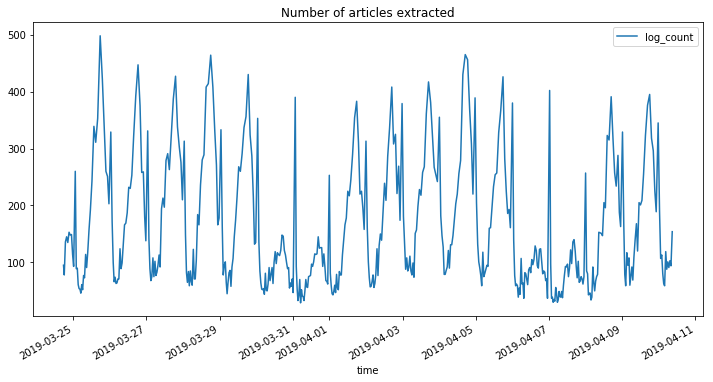
\includegraphics{log_extraction.png}\hspace*{\fill}
    
    The dataset was build only using the newspapers3k python package
    
\end{block}

%----------------------------------------------------------------------------------------
%	Dataset Properties}
%----------------------------------------------------------------------------------------

\begin{block}{Dataset Properties}

Nam quis odio enim, in molestie libero. Vivamus cursus mi at nulla elementum sollicitudin. Nam quis odio enim, in molestie libero. Vivamus cursus mi at nulla elementum sollicitudin.
  
\begin{equation}
E = mc^{2}
\label{eqn:Einstein}
\end{equation}

Nam quis odio enim, in molestie libero. Vivamus cursus mi at nulla elementum sollicitudin. Nam quis odio enim, in molestie libero. Vivamus cursus mi at nulla elementum sollicitudin.

\begin{equation}
\cos^3 \theta =\frac{1}{4}\cos\theta+\frac{3}{4}\cos 3\theta
\label{eq:refname}
\end{equation}

Nam quis odio enim, in molestie libero. Vivamus cursus mi at nulla elementum sollicitudin. Nam quis odio enim, in molestie libero. Vivamus cursus mi at nulla elementum sollicitudin.

\begin{equation}
\kappa =\frac{\xi}{E_{\mathrm{max}}} %\mathbb{ZNR}
\end{equation}

\end{block}

%----------------------------------------------------------------------------------------

\end{column} % End of column 2



\begin{column}{\sepwid}\end{column} % Empty spacer column

\begin{column}{\twocolwid} % The third column

%----------------------------------------------------------------------------------------
%	TRUMP
%----------------------------------------------------------------------------------------

\begin{block}{Trump}

\begin{columns}[onlytextwidth]
    \begin{column}{.45\textwidth}
        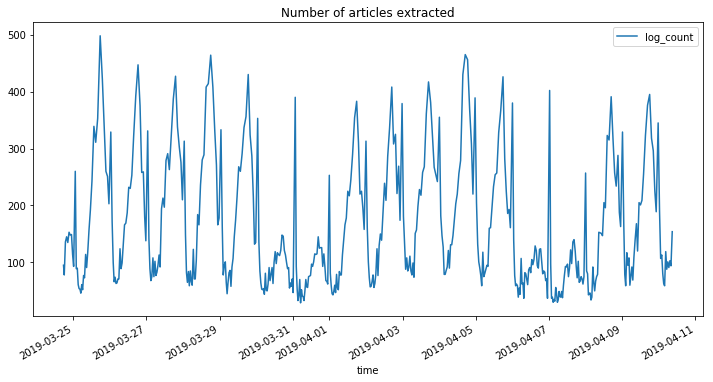
\includegraphics[width=0.8\linewidth]{log_extraction.png} 
    \end{column}
    \begin{column}{.55\textwidth}
        Fusce quis massa dictum tortor \textbf{tincidunt mattis}. Donec quam est, lobortis quis pretium at, laoreet scelerisque lacus. Nam quis odio enim, in molestie libero. Vivamus cursus mi at \textit{nulla elementum sollicitudin}.
    \end{column}
\end{columns}

\end{block}

%----------------------------------------------------------------------------------------
%	BREXIT
%----------------------------------------------------------------------------------------

\begin{block}{Brexit}


    \begin{columns}[onlytextwidth]
        \begin{column}{.55\textwidth}
            Fusce quis massa dictum tortor \textbf{tincidunt mattis}. Donec quam est, lobortis quis pretium at, laoreet scelerisque lacus. Nam quis odio enim, in molestie libero. Vivamus cursus mi at \textit{nulla elementum sollicitudin}.
        \end{column}
        \begin{column}{.45\textwidth}
            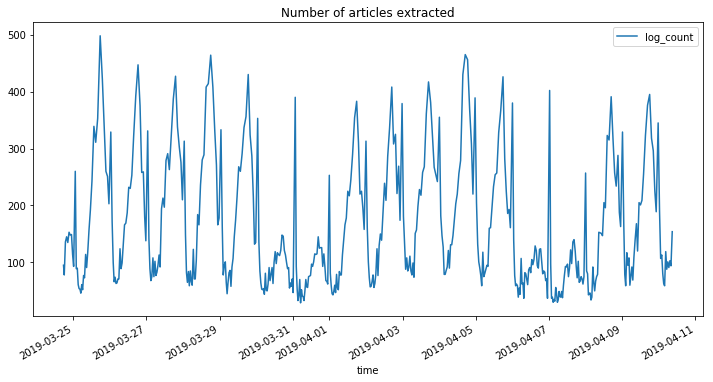
\includegraphics[width=0.8\linewidth]{log_extraction.png} 
        \end{column}
    \end{columns}

\end{block}

%----------------------------------------------------------------------------------------
%	SYRIA
%----------------------------------------------------------------------------------------

\begin{block}{Syria}
    \begin{columns}
        \begin{column}{.45\textwidth}
            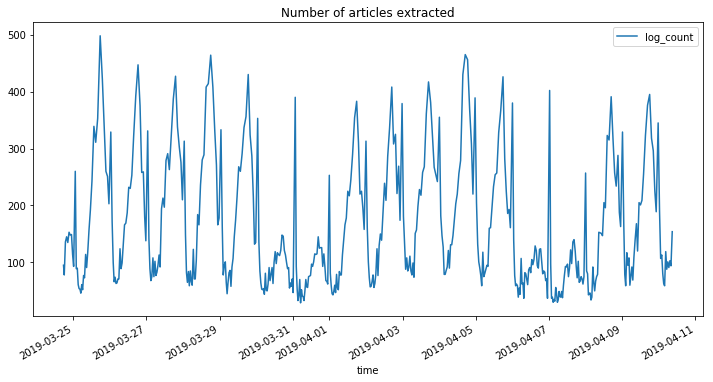
\includegraphics[width=0.8\linewidth]{log_extraction.png} 
        \end{column}
        \begin{column}{.55\textwidth}
            Fusce quis massa dictum tortor \textbf{tincidunt mattis}. Donec quam est, lobortis quis pretium at, laoreet scelerisque lacus. Nam quis odio enim, in molestie libero. Vivamus cursus mi at \textit{nulla elementum sollicitudin}.
        \end{column}
    \end{columns}
\end{block}

%----------------------------------------------------------------------------------------
%	FUTURE WORK & Conclusion
%----------------------------------------------------------------------------------------

\begin{block}{Conclusion {\emoji[ios]{1F64F}}}
    Measuring bias is a very subjective task. 
    Usually computers have a hard time executing subjective tasks. 
    The framework developed does not aim to automate bias detection but 
    rather to empower humans with summarization capabilites otherwise not possible.
    From the three example analysis above shown, it is possible to validate the usefullness of the framework proposed on a hard topic as bias detection.
    As news generation gets automated, as is the case of fakenews(needs reference), the methods of flaging them also require modern digital frameworks.
    This analysis and framework takes another step in this direction.

\end{block}


\begin{block}{Future Work {\emoji[ios]{1F64F}}}

    As previously mentioned this project aims to set a staring framework for discusion on automated detection of bias. 
    As so there is much further work to be done, mainly on 5 different areas:

    \begin{itemize}
        \item Increase the number of newspapers and find a method to select the same number of articles for each one
        \item Extrapolate the work to different regions and languages
        \item Automate topic detection 
        \item Build a ML/Rule based algorithm to flag possible high bias on articles
        \item Apply sliding window mechanimns to track changes in sentiment towards selected topics
    \end{itemize}

\end{block}


%----------------------------------------------------------------------------------------
%	REPO
%----------------------------------------------------------------------------------------

\begin{block}{ {\emoji[ios]{1F4BB}}}

    The project was possible with the great work done in the newspaper3k, nltk and gensim python libraries

    \small{\rmfamily{All code can be easily accessed in \href{https://github.com/morten-novaims/Text_Mining_HW}{github.com/morten-novaims/Text\_Mining\_HW}}} \\
    
    \end{block}

%----------------------------------------------------------------------------------------

\end{column} % End of the third column

\end{columns} % End of all the columns in the poster

\end{frame} % End of the enclosing frame

\end{document}